\newpage
\part{Misura della lunghezza d'onda della riga gialla del sodio}
\section{Finalità}
	In questa parte dell'esperienza abbiamo determinato la lunghezza d’onda $\lambda_{\text{Na}}$ della riga spettrale
	emessa da una lampada al sodio.
\section{Strumentazione}\label{sez:str_a}
	La strumentazione impiegata in questa sezione è uno spettrometro a
	prisma,riportato in \textbf{figura 1};
	tale spettroscopio si compone di:
	\begin{list}{$\cdot$}{}
		\item \textbf{una sorgente } ovvero una lampada al cadmio in fase
		di
		calibrazione e una lampada al sodio in fase di misura.
		\item \textbf{due telescopi}, uno fisso, per raccogliere la luce
		della
		sorgente e inviarla sul prisma, ed un telescopio di osservazione
		montato su di un piatto rotante e dotato di goniometro
		(sensibilità di $1/60$ di grado), in grado di ruotare
		rispetto al prisma.
		Il telescopio di raccolta  è munito di una fenditura regolabile
		attraverso la quale regolare l'ingresso della luce.

		Il telescopio di osservazione permette la regolazione del fuoco
		ed è
		inoltre regolabile attraverso delle viti.
		\item \textbf{un prisma} che costituisce l'elemento dispersivo
		dello
		spettroscopio
	\end{list}
	\bigskip
	si è inoltre impiegata una lente di ingrandimento per facilitare la
	lettura della scala del goniometro.

	\bigskip


	\begin{figure} [h]
		\centering
		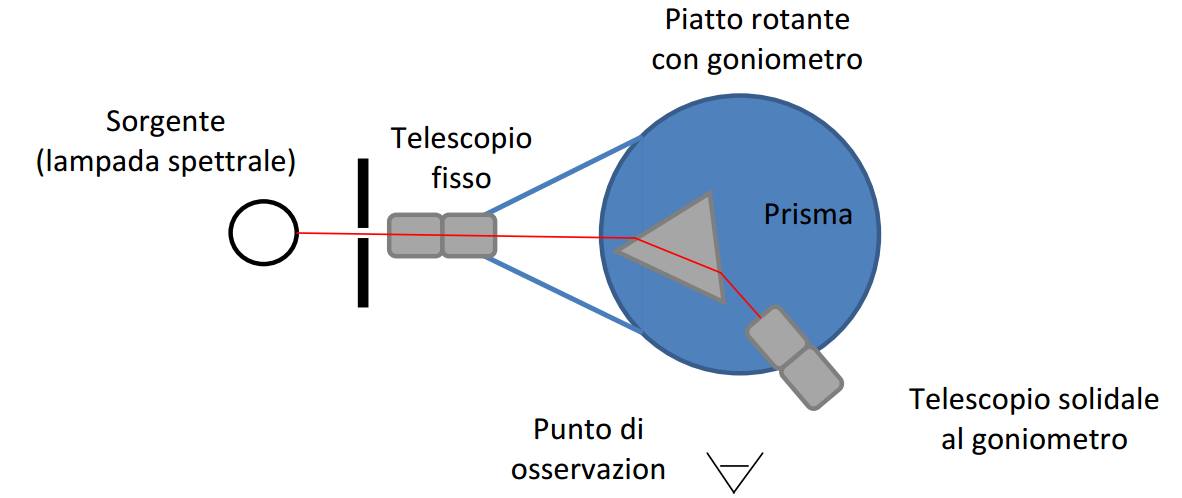
\includegraphics[width=0.9\textwidth]{./prisma}
		\caption{Schema dell'apparato impiegato.}
		\label{fig:prisma}
	\end{figure}
	Si riporta in \textbf{figura \ref{fig:prisma}} uno schema
	dell'apparato
	sperimentale impiegato.
